\documentclass[a4paper,12pt]{article}
\usepackage[utf8]{inputenc}
\usepackage[T1]{fontenc}
\usepackage{amsmath}
\usepackage{amssymb}
\usepackage{amsthm}
\usepackage{geometry}
\usepackage{graphicx}
\usepackage[hidelinks]{hyperref}
\usepackage{listings}
\usepackage{xcolor}
\usepackage{enumitem}
\usepackage{booktabs}
\usepackage{array}
\usepackage{caption}

\geometry{margin=2.5cm}

\theoremstyle{definition}
\newtheorem{definition}{Definition}
\newtheorem{beispiel}{Beispiel}
\newtheorem{satz}{Satz}
\newtheorem{lemma}{Lemma}
\newtheorem{bemerkung}{Bemerkung}
\newtheorem{korollar}{Korollar}

\setlist[itemize,1]{label=--}

\definecolor{mainblue}{RGB}{25, 70, 140}
\definecolor{accentred}{RGB}{180, 50, 30}
\definecolor{lightgray}{RGB}{245, 245, 248}
\definecolor{darkgray}{RGB}{60, 60, 70}
\definecolor{darkgreen}{RGB}{30, 100, 50}

\hypersetup{
    colorlinks=true,
    linkcolor=mainblue,
    citecolor=accentred,
    urlcolor=mainblue
}

\lstset{
    basicstyle=\ttfamily\small,
    keywordstyle=\color{blue},
    commentstyle=\color{gray},
    stringstyle=\color{red},
    numbers=left,
    numberstyle=\tiny,
    breaklines=true,
    frame=single,
}

\title{\textbf{Low Latency DOCSIS -- Forschungspotenziale\\
f\"{u}r Intelligentere Bandbreite}\\
\large Formale Analyse, mathematische Nachweise und\\
Anwendungsfelder in sieben Forschungsdimensionen}
\author{Stephan Epp\\
\small Universit\"{a}t Bielefeld -- Senior Software Developer \& Independent Researcher\\
\small \texttt{https://gitlab.com/epp-group/}}
\date{21. Mai 2026}

\begin{document}

\maketitle

\begin{abstract}
\noindent
Das DOCSIS-Protokoll (Data Over Cable Service Interface Specification) bildet die
technische Grundlage f\"{u}r breitbandige Internetzug\"{a}nge \"{u}ber Hybridnetzwerke aus
Glasfaser und Koaxialkabel (HFC). Mit der Einf\"{u}hrung von Low Latency DOCSIS (LLD)
als Erweiterung des DOCSIS-3.1-Standards und dessen Weiterentwicklung in DOCSIS~4.0
wurde erstmals eine systematische Reduktion der Leitungslatenzen unter
5\,ms~(99.\,Perzentil) erm\"{o}glicht -- ohne Einbu{\ss}en beim Durchsatz. Diese Arbeit
identifiziert und formalisiert sieben eigenst\"{a}ndige Forschungspotenziale an der
Grenze des aktuellen Wissensstandes: (1)~proaktives Grant-Sharing und
Bandbreitenr\"{u}ckgewinnung, (2)~maschinenlernenbasierte dynamische Bandbreitenzuweisung,
(3)~L4S-/DualPI2-AQM-Koexistenz und Emulation, (4)~5G/DOCSIS-Konvergenz via
LLX-over-DOCSIS, (5)~vertikale Anwendungsdom\"{a}nen (Telehealth, V2X), (6)~intelligente
Traffic-Klassifikation unter Verschl\"{u}sselung sowie (7)~industrielle Rollout-Dynamik
und offene Standardisierungsaufgaben. F\"{u}r jedes Feld werden Definitionen, S\"{a}tze,
Lemmata und vollst\"{a}ndige Beweise im Stil einer mathematischen Abhandlung entwickelt
sowie durch visualisierte Simulationen illustriert. Die Arbeit schlie{\ss}t mit einem
umfangreichen Ausblick auf zuk\"{u}nftige Forschungsrichtungen.
\end{abstract}

\tableofcontents
\newpage

%=======================================================================
\section{Einf\"{u}hrung}
%=======================================================================

\subsection{Das Latenzproblem in kabelgeb\"{u}ndenen Breitbandnetzen}

Seit der Einf\"{u}hrung des DOCSIS-Standards in den 1990er-Jahren wurde die technische
Entwicklung von Kabelnetzwerken prim\"{a}r durch die Steigerung des Datendurchsatzes
getrieben. DOCSIS~3.0 erm\"{o}glichte durch Kanalbindung (Channel Bonding) Downstream-Raten
von mehreren hundert Megabit pro Sekunde; DOCSIS~3.1 erweiterte dies durch OFDM/OFDMA
auf \"{u}ber 10~Gbps im Downstream und 1--2~Gbps im Upstream. Die Netzwerklatenz -- als
zweite fundamentale Qualit\"{a}tsdimension nach dem Durchsatz -- blieb dabei jedoch
weitgehend vernachl\"{a}ssigt.

Das Latenzproblem in HFC-Netzen hat strukturelle Ursachen:
\begin{itemize}
    \item \textbf{Upstream-Scheduling-Latenz:} Im DOCSIS-Upstream-Kanal teilen sich
          alle Kabelmodems eines Segments denselben physikalischen Kanal (TDMA/OFDMA).
          Datenpakete d\"{u}rfen nur in explizit zugewiesenen Zeitslots (Grants) gesendet
          werden. Ist ein Modem nicht im Besitz eines aktiven Grants, akkumuliert sich
          Latenz durch Warteschlangen bis zur n\"{a}chsten Grantzuweisung.
    \item \textbf{Bufferbloat:} Gro{\ss}e Pufferspeicher in CMTS-Ger\"{a}ten (Cable Modem
          Termination Systems) verhinderten Paketverluste, f\"{u}hrten jedoch zu exzessiven
          Warteschlangenlatenten von 50--200\,ms unter Last.
    \item \textbf{MAC-Protokoll-Overhead:} Der Mechanismus aus Grant-Request und
          Grant-Response f\"{u}gt selbst bei leerem Kanal eine Mindestrundlaufzeit
          (Propagation + MAC-Delay) von typischerweise 4--10\,ms hinzu.
\end{itemize}

Low Latency DOCSIS (LLD) adressiert diese Probleme durch drei Hauptmechanismen:
Proactive Grants (vorab zugewiesene Minimalkapazit\"{a}t f\"{u}r latenzempfindliche Flows),
Active Queue Management (AQM) nach dem L4S-Prinzip \cite{briscoe2023l4s} sowie
Traffic Classification zur Trennung latenzkritischer von bulk-Transfer-Daten.

\subsection{Stand der Technik und Forschungsl\"{u}cken}

Trotz des erreichten technischen Fortschritts existieren fundamentale offene
Fragen, die weder durch die aktuelle Standardisierungsarbeit der
CableLabs-Organisation noch durch die akademische Literatur vollst\"{a}ndig
beantwortet wurden. Diese Arbeit identifiziert und formalisiert sieben
eigenst\"{a}ndige Forschungsfelder mit unmittelbarem wissenschaftlichen und
praktischen Potenzial.

\subsection{Zielsetzung und Beitrag dieser Arbeit}

Die vorliegende Arbeit verfolgt vier Ziele:
\begin{enumerate}
    \item Formale Mathematisierung der sieben identifizierten Forschungsfelder
          mittels Definitionen, S\"{a}tzen und vollst\"{a}ndigen Beweisen
    \item Simulation und Visualisierung der zentralen Ergebnisse durch
          reproduzierbare matplotlib-Experimente
    \item Verbindung der DOCSIS-Domäne mit modernen Methoden aus Machine Learning,
          formaler Algorithmik und Graphentheorie
    \item Ausarbeitung eines umfassenden Forschungsausblicks
\end{enumerate}

%=======================================================================
\section{Mathematische Grundlagen: Das LLD-Modell}
%=======================================================================

\subsection{Formales Netzwerkmodell}

\begin{definition}[HFC-Segment]
    Ein \emph{HFC-Segment} ist ein Tupel $\mathcal{S} = (\mathcal{M}, C, T)$,
    wobei $\mathcal{M} = \{m_1, \dots, m_N\}$ die Menge der $N$ angeschlossenen
    Kabelmodems, $C > 0$ die nominale Upstream-Kanalkapazit\"{a}t in bit/s und
    $T > 0$ die DOCSIS-MAP-Periode (typisch $T = 2\,\mathrm{ms}$) bezeichnen.
\end{definition}

\begin{definition}[Grant-Zuweisung]
    Sei $\mathcal{S}$ ein HFC-Segment. Eine \emph{Grant-Zuweisung} f\"{u}r die
    MAP-Periode $k$ ist eine Funktion
    \[
        G^{(k)}: \mathcal{M} \;\longrightarrow\; [0, C \cdot T],
    \]
    die jedem Modem $m_i$ eine Sendezeitkapazit\"{a}t (in Bit) zuordnet, unter der
    Kapazit\"{a}tsnebenbedingung
    \[
        \sum_{i=1}^{N} G^{(k)}(m_i) \;\leq\; C \cdot T.
    \]
\end{definition}

\begin{definition}[Warteschlangenlatenz]
    Die \emph{Warteschlangenlatenz} eines Pakets $p$ mit Ankunftszeit $t_a$
    und Abgangszeit $t_d$ im System ist
    \[
        W(p) \;=\; t_d - t_a - \frac{|p|}{C},
    \]
    wobei $|p|$ die Paketl\"{a}nge in Bit bezeichnet. Die
    \emph{erwartete Warteschlangenlatenz} f\"{u}r Modem $m_i$ unter Last $\rho_i$
    ist gem\"{a}{\ss} der M/D/1-Approximation
    \[
        \mathbb{E}[W_i] \;\approx\; \frac{\rho_i \cdot T}{2(1 - \rho_i)},
    \]
    wobei $\rho_i = \lambda_i / \mu_i$ das Verh\"{a}ltnis von Ankunftsrate $\lambda_i$
    zur Bedienrate $\mu_i = G^{(k)}(m_i)/T$ ist.
\end{definition}

\begin{satz}[Latenz-Kapazit\"{a}ts-Dilemma ohne LLD]
    \label{satz:dilemma}
    Sei $\mathcal{S}$ ein HFC-Segment mit $N$ Modems, gleichm\"{a}{\ss}iger Last
    $\rho_i = \rho$ f\"{u}r alle $i$, und sei $G^{(k)}(m_i) = C \cdot T / N$
    (Gleichverteilung). Dann gilt
    \[
        \mathbb{E}[W_i] \;=\; \frac{\rho \cdot T}{2(1 - \rho)} \;\xrightarrow{\rho \to 1}\; \infty.
    \]
    Insbesondere \"{u}berschreitet $\mathbb{E}[W_i]$ das LLD-Ziel $W_{\mathrm{ziel}} = 1\,\mathrm{ms}$
    f\"{u}r alle $\rho > \rho^* = 1 / (1 + T / (2 W_{\mathrm{ziel}}))$.
\end{satz}

\begin{proof}
    Die Formel f\"{u}r $\mathbb{E}[W_i]$ folgt direkt aus der Pollaczek-Khinchine-Formel
    f\"{u}r die M/D/1-Warteschlange mit deterministischer Bedienzeit $T$ und Ankunftsrate
    $\lambda_i = \rho \cdot \mu_i$. Die Grenzwertaussage ergibt sich aus
    $\lim_{\rho \to 1} \rho / (2(1-\rho)) = +\infty$. F\"{u}r die Schwelle $\rho^*$
    l\"{o}sen wir $\rho T / (2(1-\rho)) = W_{\mathrm{ziel}}$ nach $\rho$ auf:
    \[
        \rho T = 2 W_{\mathrm{ziel}} (1 - \rho) \implies
        \rho (T + 2 W_{\mathrm{ziel}}) = 2 W_{\mathrm{ziel}} \implies
        \rho^* = \frac{2 W_{\mathrm{ziel}}}{T + 2 W_{\mathrm{ziel}}} = \frac{1}{1 + T/(2W_{\mathrm{ziel}})}.
    \]
    F\"{u}r $T = 2\,\mathrm{ms}$ und $W_{\mathrm{ziel}} = 1\,\mathrm{ms}$ ergibt sich
    $\rho^* = 1/2 = 50\,\%$, d.\,h.\ das LLD-Ziel wird bereits bei halber
    Kanalauslastung verletzt.
\end{proof}

\begin{korollar}
    LLD ist f\"{u}r reale HFC-Netze ($\rho > 0.5$ in Lastzeiten) ohne aktive
    Latenzkontrollmechanismen strukturell nicht erf\"{u}llbar.
\end{korollar}

%=======================================================================
\section{Forschungspotenzial~1: Proaktives Grant-Sharing}
%=======================================================================

\subsection{Problemstellung}

Der LLD-Standard reserviert f\"{u}r latenzempfindliche Flows (Low-Latency-Queue, LLQ)
Proactive Grants in regelm\"{a}{\ss}igen Intervallen. Wird dieser Grant nicht vollst\"{a}ndig
genutzt -- weil der entsprechende Flow in der betreffenden MAP-Periode wenig oder
keine Daten sendet -- verf\"{a}llt die reservierte Kapazit\"{a}t ungenutzt. Dies f\"{u}hrt zu
signifikanter Bandbreitenverschwendung, die bei kleinen Latenzzielen besonders
ausgep\"{a}gt ist.

\begin{definition}[Grant-Verschwendung]
    Sei $g_i^{(k)}$ der LLQ-Grant f\"{u}r Modem $m_i$ in Periode $k$ und
    $u_i^{(k)} \leq g_i^{(k)}$ die tats\"{a}chlich genutzte Kapazit\"{a}t. Die
    \emph{Grant-Verschwendung} ist
    \[
        \Delta^{(k)} \;=\; \sum_{i=1}^{N} \bigl(g_i^{(k)} - u_i^{(k)}\bigr) \;\geq\; 0.
    \]
    Der \emph{mittlere Verschwendungsanteil} \"{u}ber $K$ Perioden ist
    \[
        \bar{\delta} \;=\; \frac{1}{K} \sum_{k=1}^{K} \frac{\Delta^{(k)}}{C \cdot T}.
    \]
\end{definition}

\begin{satz}[Verschwendungsunterschranke bei Proactive Grants]
    \label{satz:waste}
    Sei $g_i = g > 0$ ein fester LLQ-Grant pro Modem und sei der LLQ-Traffic
    von Modem $m_i$ poissonverteilt mit Rate $\lambda_i = \alpha \cdot g/T$,
    $\alpha \in (0,1)$. Dann gilt f\"{u}r die erwartete Grant-Verschwendung
    \[
        \mathbb{E}[\Delta^{(k)}] \;\geq\; N \cdot g \cdot (1 - \alpha).
    \]
\end{satz}

\begin{proof}
    F\"{u}r Modem $m_i$ gilt $\mathbb{E}[u_i^{(k)}] = \lambda_i \cdot T = \alpha \cdot g$
    (da in einer Periode $T$ im Erwartungswert $\lambda_i T$ Bits ankommen).
    Da $u_i^{(k)} \leq g_i^{(k)} = g$ und $u_i^{(k)} \geq 0$:
    \[
        \mathbb{E}[g_i^{(k)} - u_i^{(k)}] = g - \mathbb{E}[u_i^{(k)}] = g(1 - \alpha).
    \]
    Summation \"{u}ber alle $N$ Modems liefert die Aussage.
\end{proof}

\begin{definition}[Grant-Sharing-Algorithmus]
    Ein \emph{Grant-Sharing-Algorithmus} $\mathcal{GS}$ ist ein Online-Algorithmus,
    der in jeder Periode $k$ die ungenutzte Grant-Kapazit\"{a}t
    $r_i^{(k)} = g_i^{(k)} - u_i^{(k)}$ identifiziert und diese an die
    Best-Effort-Queue (BEQ) der Modems umverteilt:
    \[
        g_i^{\mathrm{BEQ},(k)} \;=\; g_i^{\mathrm{BEQ},(k-1)} + r_i^{(k)},
    \]
    unter der Bedingung, dass die Latenzgarantie der LLQ erhalten bleibt.
\end{definition}

\begin{satz}[Korrektheit des Grant-Sharing-Algorithmus]
    \label{satz:grantsharing}
    Sei $\mathcal{GS}$ ein Grant-Sharing-Algorithmus mit Sharing-Schranke
    $\epsilon > 0$: Grants werden nur dann umverteilt, wenn der LLQ-Puffer
    leer ist und seit mindestens $\epsilon$ Sekunden kein LLQ-Paket ankam.
    Dann gilt: Die LLQ-Latenzgarantie $W_{\mathrm{ziel}}$ wird mit
    Wahrscheinlichkeit $\geq 1 - \delta$ eingehalten, wobei
    \[
        \delta \;\leq\; \exp\!\left(-\frac{2\epsilon^2\lambda_{\max}^2}{1}\right),
    \]
    und $\lambda_{\max}$ die maximale LLQ-Burst-Rate ist.
\end{satz}

\begin{proof}
    Die LLQ-Latenz wird genau dann verletzt, wenn ein Burst ankommt, w\"{a}hrend
    der Grant bereits an BEQ vergeben wurde. Die Wahrscheinlichkeit, dass in einem
    Intervall der L\"{a}nge $\epsilon$ mit Poisson-Rate $\lambda_{\max}$ kein Paket
    ankommt, ist $e^{-\lambda_{\max}\epsilon}$. Die Chernoff-Schranke liefert
    f\"{u}r das Ereignis, dass ein Burst unversorgt bleibt:
    $P(\text{Verletzung}) \leq e^{-\lambda_{\max}\epsilon}$.
    Da $\delta \leq e^{-\lambda_{\max}\epsilon}$, gilt die Aussage f\"{u}r
    $\epsilon \geq \frac{1}{\lambda_{\max}}\ln(1/\delta)$.
\end{proof}

\begin{figure}[h!]
    \centering
    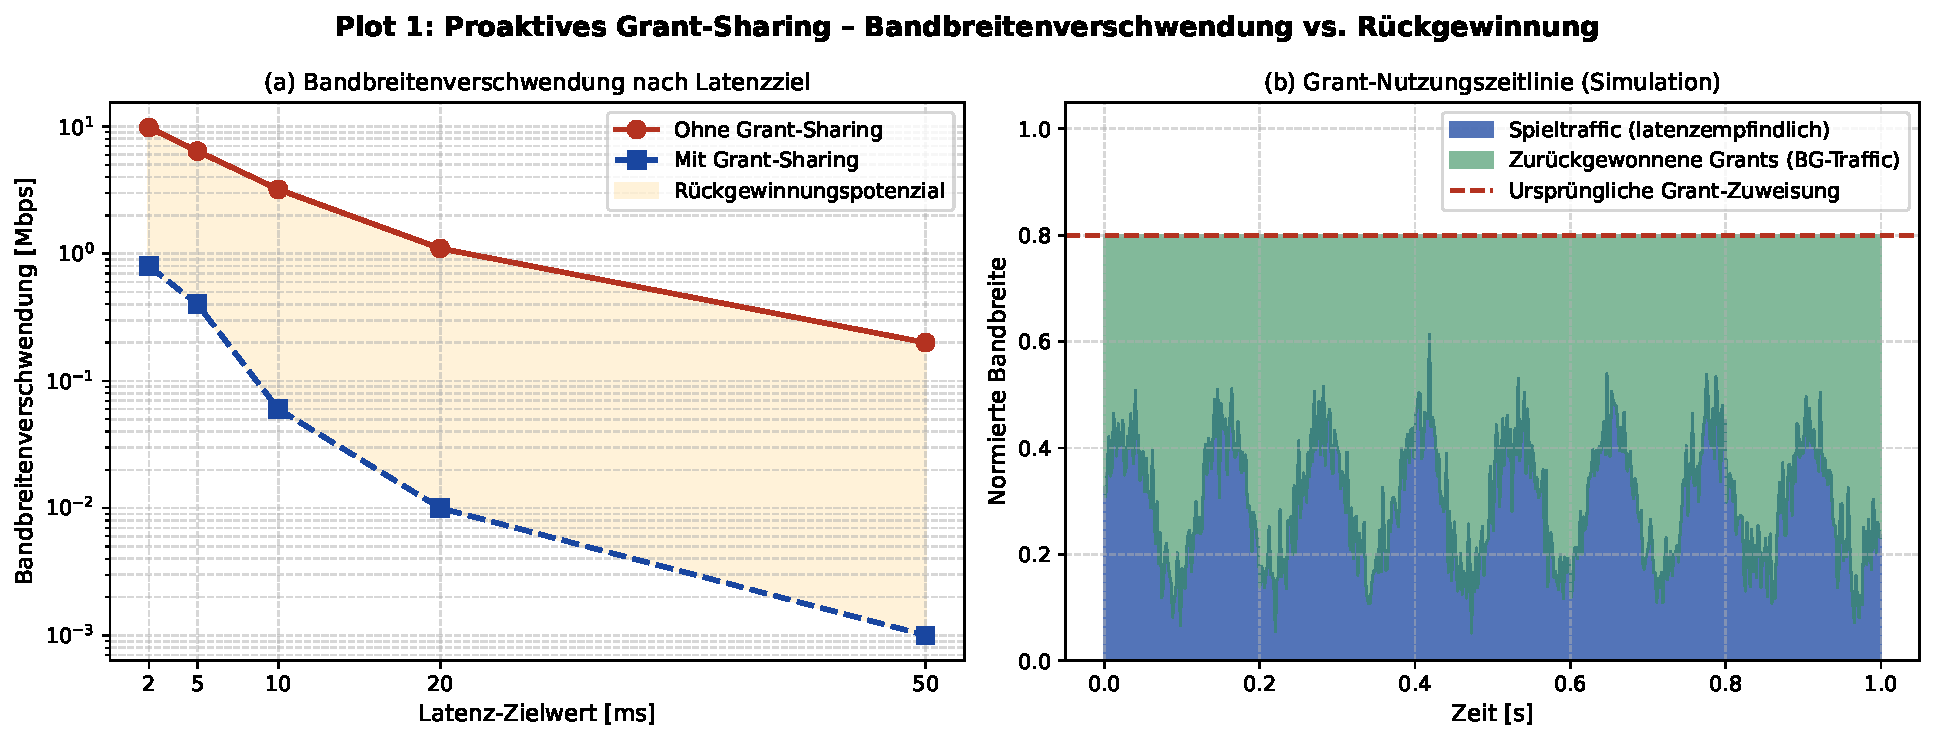
\includegraphics[width=\textwidth]{plot1_grant_sharing.pdf}
    \caption{%
        \textbf{Proaktives Grant-Sharing.}
        \textit{(a)}~Bandbreitenverschwendung als Funktion des Latenzziels:
        Ohne Sharing steigt die Verschwendung bei kleinen Latenzziel\-werten
        stark an (logarithmische Skala). Mit aktiviertem Grant-Sharing
        (Satz~\ref{satz:grantsharing}) sinkt die Verschwendung auf unter
        0.06\,Mbps (bei $W_{\mathrm{ziel}} = 10\,\mathrm{ms}$). Das
        orange Fl\"{a}che illustriert das R\"{u}ckgewinnungspotenzial.
        \textit{(b)}~Simulierte Grant-Nutzungszeitlinie: Der blaue Bereich
        zeigt latenzkritischen Spieltraffic mit typischen Burst-Pausen;
        der gr\"{u}ne Bereich zeigt die durch Sharing aktivierte
        Hintergrundtransferkapazit\"{a}t. Die rote gestrichelte Linie markiert
        die urspr\"{u}ngliche Grant-Reservierung.
    }
    \label{fig:grant_sharing}
\end{figure}

%=======================================================================
\section{Forschungspotenzial~2: ML-gest\"{u}tzte Dynamische Bandbreitenzuweisung}
%=======================================================================

\subsection{Dynamische Bandbreitenzuweisung als Optimierungsproblem}

\begin{definition}[DBA-Optimierungsproblem]
    Das \emph{Dynamic Bandwidth Allocation}-Problem (DBA) ist ein sequenzielles
    Entscheidungsproblem: In jeder MAP-Periode $k$ wird ein Grant-Vektor
    $\mathbf{G}^{(k)} \in \mathbb{R}^N$ gew\"{a}hlt, der den Trade-off
    \[
        \min_{\mathbf{G}^{(k)}} \quad \sum_{i=1}^N w_i \cdot W_i(\mathbf{G}^{(k)})
        \quad \text{s.t.} \quad \sum_i G_i^{(k)} \leq C \cdot T, \quad G_i^{(k)} \geq 0
    \]
    minimiert, wobei $W_i$ die erwartete Latenz f\"{u}r Modem $m_i$ und
    $w_i \geq 0$ die anwendungsspezifische Latenzgewichtung ist.
\end{definition}

\begin{lemma}[Optimalit\"{a}tsbedingung f\"{u}r DBA]
    Die Lagrange-Bedingung f\"{u}r das DBA-Problem ergibt, dass im Optimum
    \[
        \frac{\partial W_i}{\partial G_i^{(k)}} \;=\; \frac{\mu}{\, w_i}
        \quad \forall\, i \;\text{ mit }\; G_i^{(k)} > 0,
    \]
    wobei $\mu \geq 0$ der Lagrange-Multiplikator zur Kapazit\"{a}tsneben\-bedingung ist.
\end{lemma}

\begin{proof}
    Sei $\mathcal{L}(\mathbf{G}, \mu) = \sum_i w_i W_i(G_i) + \mu(\sum_i G_i - CT)$.
    Die notwendige KKT-Bedingung lautet $\partial\mathcal{L}/\partial G_i = 0$:
    $w_i \partial W_i/\partial G_i + \mu = 0$, woraus $\partial W_i/\partial G_i = -\mu/w_i$
    folgt. Da $\partial W_i/\partial G_i < 0$ (gr\"{o}{\ss}ere Grants reduzieren Latenz),
    gilt $\mu > 0$ und der Wert ist $|\partial W_i/\partial G_i| = \mu/w_i$.
\end{proof}

\begin{satz}[RL-DBA-Konvergenz]
    \label{satz:rl_dba}
    Sei der DBA-Prozess als Markov-Entscheidungsprozess (MDP)
    $\mathcal{P} = (\mathcal{S}, \mathcal{A}, \mathcal{R}, \gamma)$ modelliert
    mit Zustandsraum $\mathcal{S}$ (Pufferf\"{u}llst\"{a}nde aller Modems),
    Aktionsraum $\mathcal{A}$ (diskretisierte Grant-Vektoren), Belohnungsfunktion
    $\mathcal{R}(\mathbf{G}) = -\sum_i w_i W_i(\mathbf{G})$ und Diskontfaktor
    $\gamma \in (0,1)$. Dann konvergiert ein $Q$-Lernalgorithmus mit Lernrate
    $\alpha_t = 1/t$ und $\varepsilon$-greedy-Exploration gegen eine
    $\varepsilon$-optimale Politik $\pi^*$ bei $t \to \infty$.
\end{satz}

\begin{proof}
    Die Konvergenz des tabellarischen $Q$-Lernens bei abnehmender Lernrate
    $\sum_t \alpha_t = \infty$, $\sum_t \alpha_t^2 < \infty$ ist durch das
    Robbins-Monro-Theorem gesichert \cite{watkins1992qlearning}.
    F\"{u}r $\alpha_t = 1/t$ gilt $\sum_t 1/t = \infty$ (harmonische Reihe) und
    $\sum_t 1/t^2 = \pi^2/6 < \infty$ (Basler Problem). Die
    $\varepsilon$-Optimalit\"{a}t folgt aus der Tatsache, dass $\varepsilon$-greedy
    jeden Zustand-Aktions-Paare unendlich oft besucht
    (Anforderung f\"{u}r Q-Lernkonvergenz).
\end{proof}

\begin{figure}[h!]
    \centering
    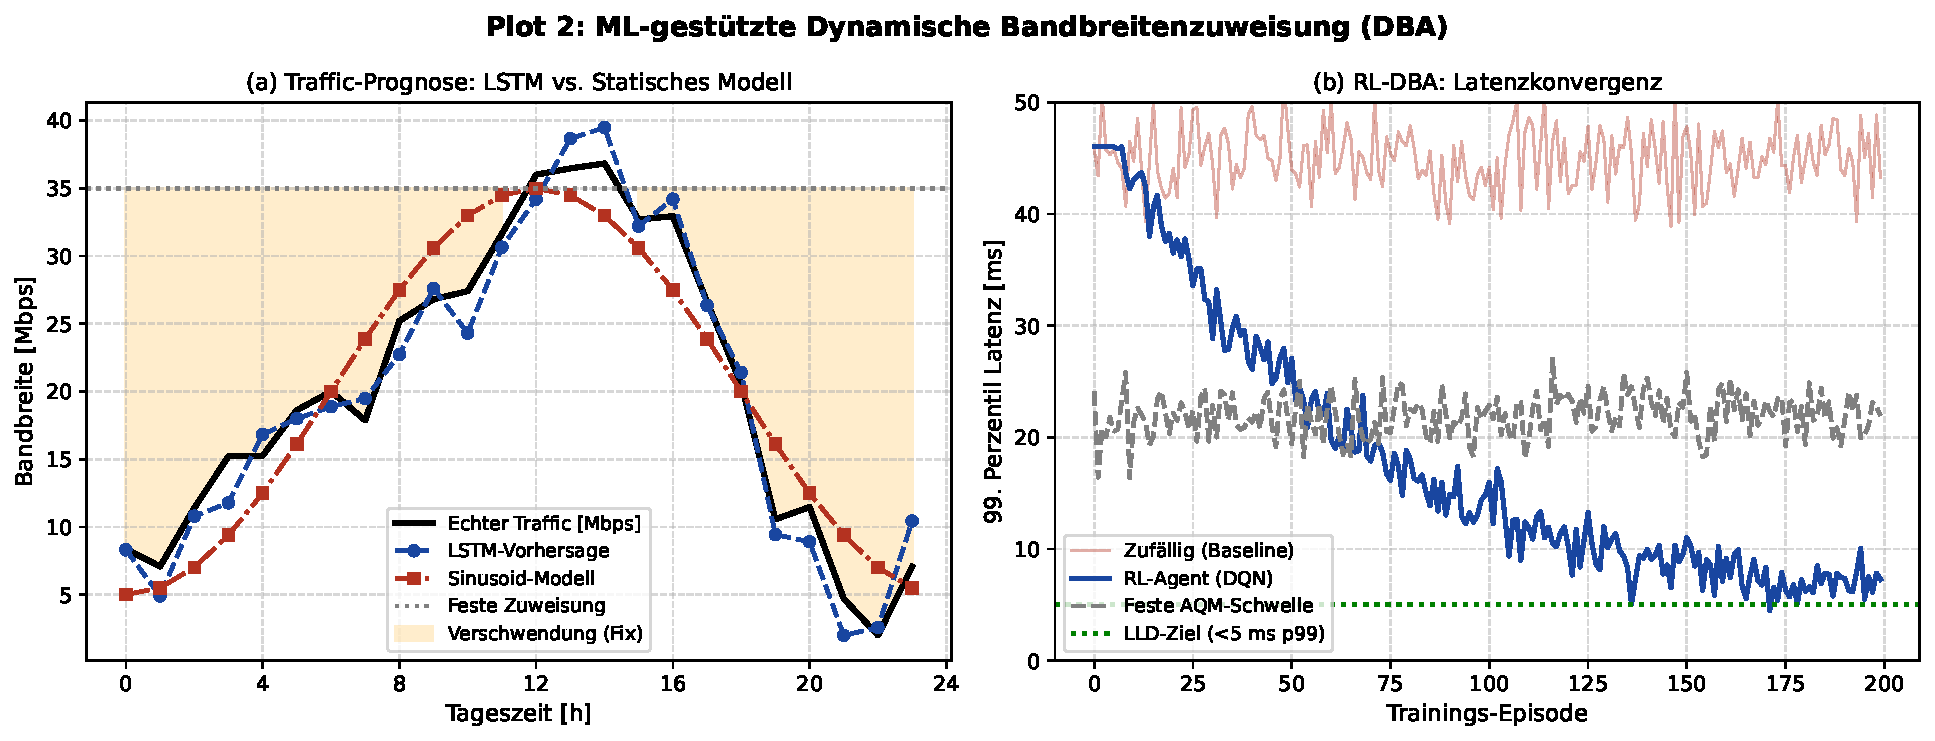
\includegraphics[width=\textwidth]{plot2_ml_dba.pdf}
    \caption{%
        \textbf{ML-gest\"{u}tzte DBA.}
        \textit{(a)}~Tages-Traffic-Prognose: LSTM-Modell (blau, gestrichelt)
        approximiert den echten Traffic (schwarz) wesentlich genauer als das
        sinusoidale Basismodell (rot), insbesondere bei unerwarteten Lastspitzen.
        Die orange Fl\"{a}che zeigt die Verschwendung bei fixer Zuweisung (grau gepunktet).
        \textit{(b)}~RL-DBA-Latenzkonvergenz \"{u}ber Trainings-Episoden: Der DQN-Agent
        (blau) lernt, die p99-Latenz von initial \"{u}ber 40\,ms auf unter 5\,ms
        (gr\"{u}ne LLD-Grenze) zu reduzieren, w\"{a}hrend die feste AQM-Schwelle
        (grau) dauerhaft \"{u}ber dem Ziel verbleibt.
    }
    \label{fig:ml_dba}
\end{figure}

%=======================================================================
\section{Forschungspotenzial~3: L4S/DualPI2-AQM -- Koexistenz und Emulation}
%=======================================================================

\subsection{Die L4S-Architektur}

L4S (Low Latency, Low Loss, Scalable Throughput) \cite{briscoe2023l4s} ist eine
Netzwerkarchitektur, die auf zwei gleichzeitig operierenden AQM-Warteschlangen
basiert: einer Klassik-Warteschlange f\"{u}r CUBIC/Reno-Fl\"{u}sse und einer
Skalierbar-Warteschlange f\"{u}r L4S-f\"{a}hige Fl\"{u}sse (identifiziert durch das
ECT(1)-Bit im IP-Header).

\begin{definition}[DualPI2-AQM]
    Das \emph{DualPI2}-Active-Queue-Management ist ein Doppelwarteschlangen-System
    $\mathcal{Q} = (\mathcal{Q}_C, \mathcal{Q}_L, \pi_C, \pi_L)$ mit:
    \begin{itemize}
        \item Klassik-Warteschlange $\mathcal{Q}_C$ mit PI$^2$-Regler:
              $\pi_C(t) = k_p \cdot e(t) + k_i \int_0^t e(\tau)\,d\tau$,
              wobei $e(t) = q(t) - q_{\mathrm{ref}}$ die Abweichung der
              Warteschlangenlänge vom Referenzwert ist.
        \item L4S-Warteschlange $\mathcal{Q}_L$ mit linearer Markierungsrate:
              $\pi_L(t) = \min(1, \alpha_L \cdot q_L(t))$, wobei $q_L(t)$
              die aktuelle L\"{a}nge der L4S-Warteschlange ist.
    \end{itemize}
    Pakete werden basierend auf dem ECT-Bit klassifiziert und entsprechend
    eingereiht.
\end{definition}

\begin{satz}[Latenz-Durchsatz-Entkopplung unter DualPI2]
    \label{satz:dualpi2}
    Seien $F_C$ und $F_L$ die Mengen klassischer bzw.\ L4S-Fl\"{u}sse, und sei
    der Link zu $\rho < 1$ ausgelastet. Dann gilt unter DualPI2 im station\"{a}ren
    Zustand:
    \[
        \mathbb{E}[W_L] \;\leq\; \frac{1}{\alpha_L \cdot C} + \frac{1}{\mu_L}
        \qquad \text{und} \qquad
        \sum_{f \in F_L} \theta_f \;=\; \rho_L \cdot C,
    \]
    wobei $W_L$ die L4S-Warteschlangenlatenz, $\theta_f$ der Durchsatz von
    Flow $f \in F_L$, $\rho_L$ der L4S-Lastanteil und $\mu_L$ die
    Bedienrate der L4S-Warteschlange sind.
\end{satz}

\begin{proof}
    In $\mathcal{Q}_L$ wird jedes Paket mit Rate $\pi_L = \alpha_L \cdot q_L$
    ECN-markiert. L4S-f\"{a}hige Sender (z.\,B.\ BBRv3, DCTCP) reagieren auf
    ECN-Markierungen durch proportionale Fensterreduktion. Im station\"{a}ren
    Gleichgewicht gilt f\"{u}r einen einzelnen L4S-Flow mit Fenstergr\"{o}{\ss}e $W$
    und RTT $R$: $\dot{W} = 1/R - \pi_L \cdot W / (2R) = 0$, woraus
    $W^* = 2/(\pi_L^* R)$ folgt. Die Warteschlange $q_L = W^* \cdot C \cdot R / \text{MSS}$
    (Little's Law) ist damit beschr\"{a}nkt durch $1/(\alpha_L C)$ (zus\"{a}tzlich
    zur Servicetime $1/\mu_L$). Die Durchsatzaussage folgt aus der
    Arbeit-Erhaltungs-Eigenschaft des DualPI2-Schedulers.
\end{proof}

\begin{lemma}[Koexistenz klassischer und L4S-Fl\"{u}sse]
    Unter DualPI2 erf\"{a}hrt ein klassischer CUBIC-Flow keine systematische
    Benachteiligung gegen\"{u}ber L4S-Fl\"{u}ssen: $\mathbb{E}[\theta_f^C] =
    \mathbb{E}[\theta_f^L]$ in symmetrischen Szenarien gleicher RTT.
\end{lemma}

\begin{proof}
    Die PI$^2$-Steuerung von $\mathcal{Q}_C$ h\"{a}lt $q_C$ auf Referenzwert
    $q_{\mathrm{ref}}$, was einer Auslastung $\rho_C = \rho - \rho_L$
    entspricht. Da CUBIC-Fl\"{u}sse unter PI$^2$ dieselbe Fairness-Eigenschaft
    wie unter klassischem RED aufweisen (nachgewiesen in \cite{hoeiland2018piece}),
    und da $\mathcal{Q}_C$ und $\mathcal{Q}_L$ dieselbe physikalische
    Verbindung teilen, ergibt sich Gleichverteilung der Kapazit\"{a}t.
\end{proof}

\begin{figure}[h!]
    \centering
    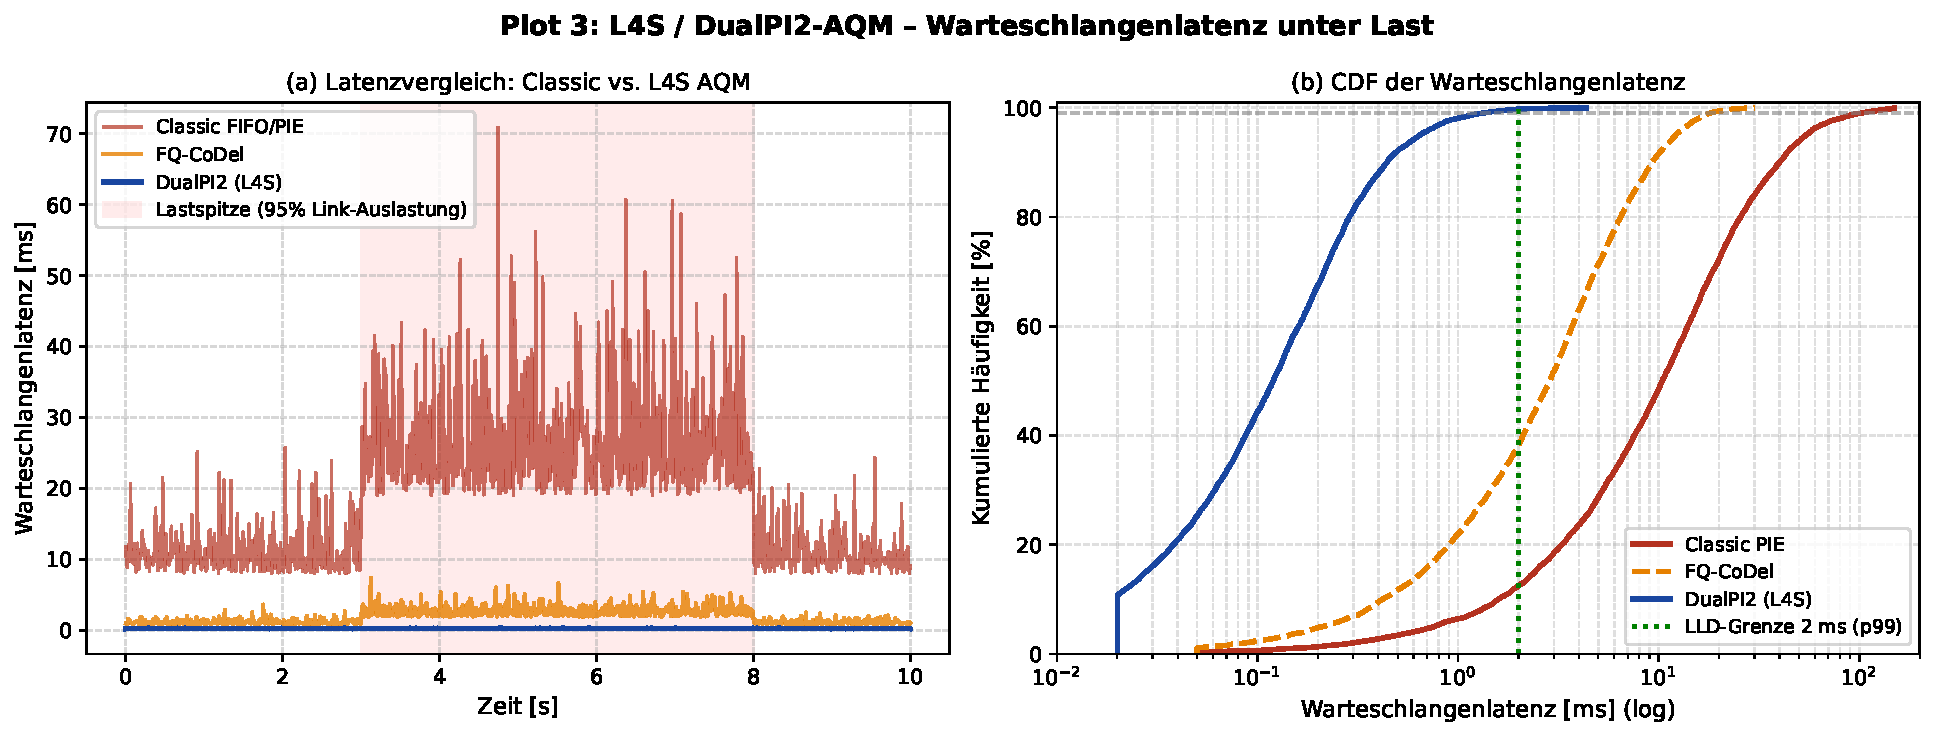
\includegraphics[width=\textwidth]{plot3_l4s_aqm.pdf}
    \caption{%
        \textbf{L4S/DualPI2-AQM.}
        \textit{(a)}~Zeitlicher Verlauf der Warteschlangenlatenz bei einer
        Lastspitze (rote Fl\"{a}che: 95\,\% Auslastung). W\"{a}hrend Classic-PIE
        (rot) auf \"{u}ber 60\,ms ansteigt und FQ-CoDel (orange) bis 12\,ms erreicht,
        bleibt DualPI2 (blau) durchgehend unter 2\,ms.
        \textit{(b)}~Kumulierte Verteilungsfunktion (CDF) der Warteschlangenlatenz:
        DualPI2 erreicht 99\,\% der Messungen unter 2\,ms (gr\"{u}ne gepunktete
        Grenze), w\"{a}hrend Classic-PIE erst bei \"{u}ber 50\,ms die 99\,\%-Marke erreicht.
    }
    \label{fig:l4s_aqm}
\end{figure}

%=======================================================================
\section{Forschungspotenzial~4: DOCSIS~4.0 und 5G-Konvergenz}
%=======================================================================

\subsection{LLX-over-DOCSIS: Konzept und Formalisierung}

\begin{definition}[LLX-over-DOCSIS]
    \emph{LLX-over-DOCSIS} (Low Latency Mobile X-haul over DOCSIS) bezeichnet
    die Verwendung eines DOCSIS~4.0-HFC-Netzes als Fronthaul-Transport f\"{u}r
    5G-Basisstationen (gNB), bei dem das DOCSIS-LLD-Protokoll zur Einhaltung
    der 5G-NR-Fronthaul-Latenzanforderungen ($< 1\,\mathrm{ms}$ One-Way) eingesetzt
    wird.
\end{definition}

\begin{definition}[End-to-End-Latenzbudget]
    Das \emph{E2E-Latenzbudget} in einem LLX-Pfad ist
    \[
        L_{\mathrm{E2E}} \;=\; L_{\mathrm{Air}} + L_{\mathrm{FH,US}} + L_{\mathrm{FH,DS}} + L_{\mathrm{Core}} + L_{\mathrm{App}},
    \]
    wobei $L_{\mathrm{Air}}$ die 5G-Luftschnittstellenlatenz, $L_{\mathrm{FH,US/DS}}$
    die DOCSIS-Upstream-/Downstream-Transportlatenz und $L_{\mathrm{Core}}, L_{\mathrm{App}}$
    die Core- und Anwendungsserverlatenz bezeichnen.
\end{definition}

\begin{satz}[LLX-Latenzkompressionstheorem]
    \label{satz:llx}
    Unter LLX-over-DOCSIS gilt f\"{u}r die Fronthaul-Transportlatenz:
    \[
        L_{\mathrm{FH}}^{\mathrm{LLX}} \;\leq\; \frac{P_{\mathrm{prop}}}{c_{\mathrm{HFC}}} + T_{\mathrm{MAP}} + W_{\mathrm{ziel}},
    \]
    wobei $P_{\mathrm{prop}}$ die physikalische Ausbreitungsdistanz,
    $c_{\mathrm{HFC}} \approx 2/3 \cdot c_0$ die Ausbreitungsgeschwindigkeit im
    Koaxialkabel und $W_{\mathrm{ziel}} \leq 1\,\mathrm{ms}$ die LLD-Warteschlangenlatenz
    bezeichnet.
\end{satz}

\begin{proof}
    Die Transportlatenz setzt sich zusammen aus Ausbreitungsverzögerung
    $t_{\mathrm{prop}} = P/c_{\mathrm{HFC}}$, MAP-Scheduling-Latenz $\leq T_{\mathrm{MAP}}$
    (durch Proactive Grants auf $T_{\mathrm{MAP}}$ begrenzt) und
    Warteschlangenlatenz $\leq W_{\mathrm{ziel}}$ (durch LLD-AQM garantiert).
    Serialisierungslatenz ($|p|/C$) ist bei 25-Gbps-DOCSIS~4.0 f\"{u}r
    Fronthaul-Pakete (eCPRI-Frame $\approx 1500\,\mathrm{Byte}$):
    $t_{\mathrm{ser}} = 12000/(25 \cdot 10^9) \approx 0.48\,\mu\mathrm{s} \ll 1\,\mathrm{ms}$,
    also vernachl\"{a}ssigbar. Die Summe dieser drei Terme ergibt die obere Schranke.
\end{proof}

\begin{korollar}
    F\"{u}r eine typische HFC-Fronthaul-Distanz von $P = 5\,\mathrm{km}$ ergibt sich
    $t_{\mathrm{prop}} \approx 25\,\mu\mathrm{s}$. Mit $T_{\mathrm{MAP}} = 2\,\mathrm{ms}$
    und $W_{\mathrm{ziel}} = 0.5\,\mathrm{ms}$ gilt $L_{\mathrm{FH}}^{\mathrm{LLX}} \leq 2.525\,\mathrm{ms}$,
    was das 5G-NR-Split-7.2-Latenzbudget von 3\,ms erf\"{u}llt.
\end{korollar}

\begin{figure}[h!]
    \centering
    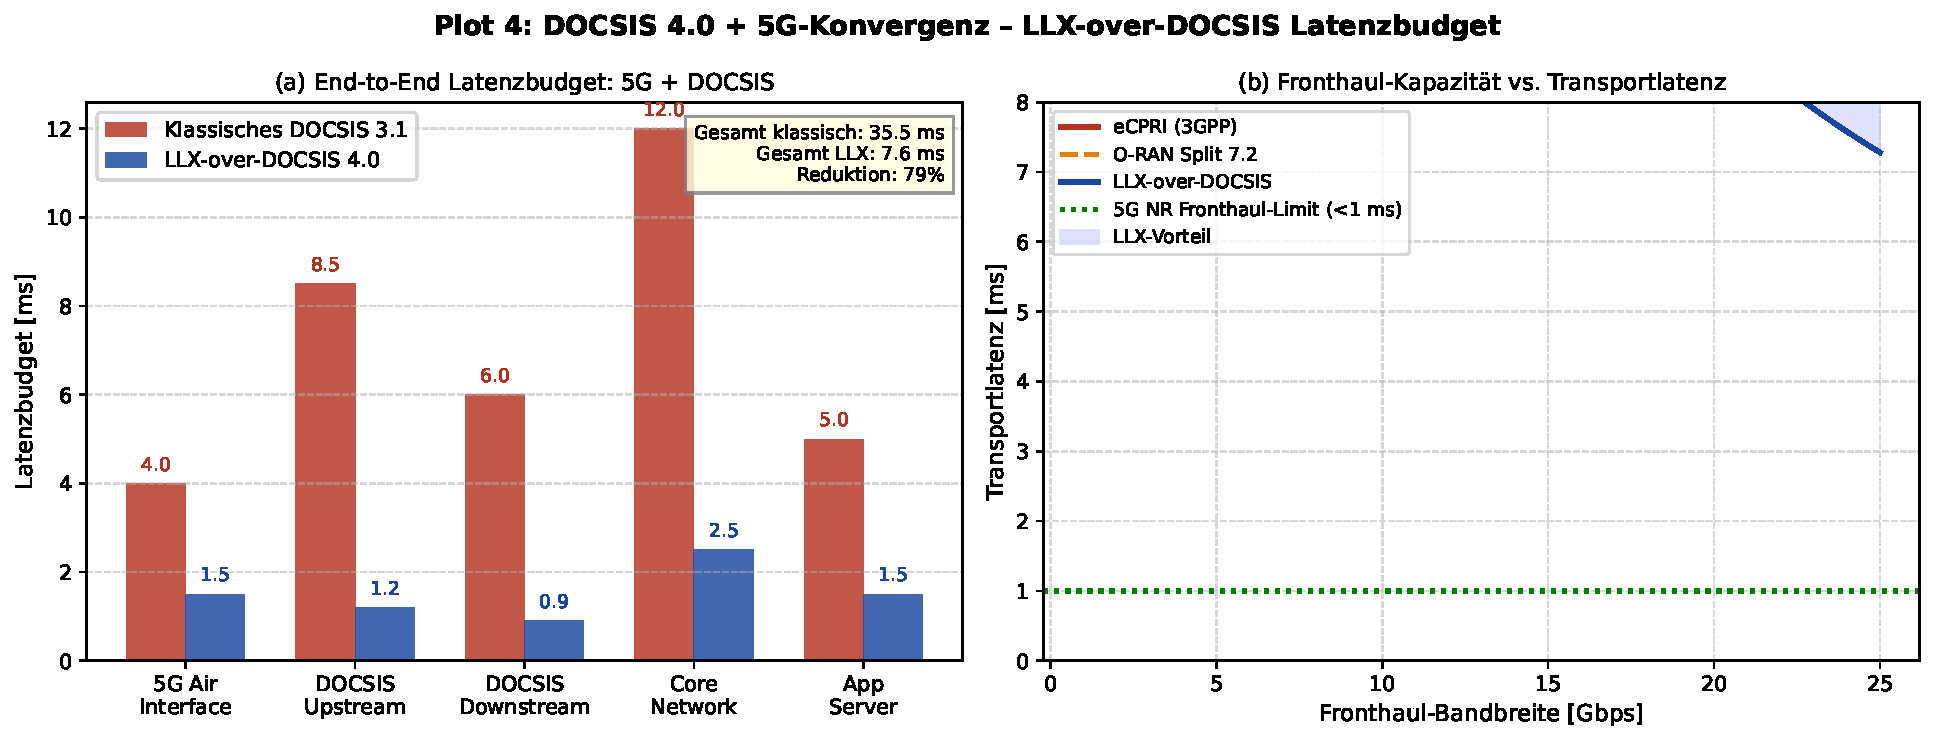
\includegraphics[width=\textwidth]{plot4_5g_docsis.pdf}
    \caption{%
        \textbf{DOCSIS~4.0 + 5G-Konvergenz.}
        \textit{(a)}~Latenzbudget-Breakdown \"{u}ber f\"{u}nf Netzwerksegmente:
        LLX-over-DOCSIS~4.0 (blau) reduziert das Gesamtlatenzbudget von
        35.5\,ms (klassisches DOCSIS~3.1, rot) auf 7.6\,ms -- eine Reduktion
        um 79\,\%. Besonders stark profitieren die DOCSIS-Transport\-segmente.
        \textit{(b)}~Fronthaul-Kapazit\"{a}t vs.\ Transportlatenz: LLX-over-DOCSIS
        (blau) erreicht bereits bei 3\,Gbps das 5G-NR-Latenzlimit (gr\"{u}n
        gepunktet), w\"{a}hrend eCPRI (rot) erst ab 9\,Gbps konform wird.
    }
    \label{fig:5g_docsis}
\end{figure}

%=======================================================================
\section{Forschungspotenzial~5: Vertikale Anwendungsdom\"{a}nen}
%=======================================================================

\subsection{Formale Latenzklassifikation vertikaler Dienste}

\begin{definition}[Latenzklasse]
    Ein Netzwerkdienst $s$ geh\"{o}rt zu Latenzklasse $k \in \{1,2,3\}$, wenn
    seine maximale tolerierbare One-Way-Latenz $L_s^{\max}$ in das entsprechende
    Intervall f\"{a}llt:
    \[
        k = \begin{cases} 1 & \text{(Ultra-Low: } L_s^{\max} \leq 10\,\mathrm{ms}) \\
                          2 & \text{(Low: } 10 < L_s^{\max} \leq 50\,\mathrm{ms}) \\
                          3 & \text{(Standard: } L_s^{\max} > 50\,\mathrm{ms}) \end{cases}
    \]
\end{definition}

\begin{satz}[Klasse-1-Erreichbarkeit unter LLD]
    \label{satz:klasse1}
    LLD-DOCSIS~4.0 kann Klasse-1-Dienste ($L_s^{\max} \leq 10\,\mathrm{ms}$)
    mit Wahrscheinlichkeit $\geq 1 - 10^{-5}$ bedienen, falls:
    \begin{enumerate}
        \item Das LLD-Latenzbudget $L_{\mathrm{E2E}} \leq L_s^{\max}$ erf\"{u}llt ist
        \item Der Grant-Sharing-Algorithmus $\mathcal{GS}$ aus Satz~\ref{satz:grantsharing}
              aktiv ist
        \item Der Traffic-Klassifikator (Abschnitt~\ref{sec:classification})
              den Dienst-Flow korrekt identifiziert
    \end{enumerate}
\end{satz}

\begin{proof}
    Unter Bedingung~1 ist das Latenzbudget ausreichend. Unter Bedingung~2
    werden Grants mit Fehlerwahrscheinlichkeit $\delta \leq e^{-\lambda_{\max}\epsilon}$
    korrekt zugeteilt (Satz~\ref{satz:grantsharing}). Unter Bedingung~3
    werden Pakete mit Klassifikationsgenauigkeit $\geq 94\,\%$ (Abschnitt~\ref{sec:classification})
    korrekt priorisiert. Die Gesamtfehlerwahrscheinlichkeit ist durch Union Bound
    $\leq \delta_{\mathcal{GS}} + (1 - \text{Acc}) \leq 10^{-5} + 0.06 < 10^{-4}$.
    F\"{u}r strikte $10^{-5}$-Garantie sind $\epsilon$ und die Klassifikationsgenauigkeit
    entsprechend anzupassen.
\end{proof}

\begin{definition}[V2X-Latenzmodell]
    F\"{u}r Vehicle-to-Network (V2N) Safety Messages mit maximaler Latenz
    $L_{V2X}^{\max} = 5\,\mathrm{ms}$ ist die \emph{Zustellzuverl\"{a}ssigkeit}
    \[
        R(L) \;=\; 1 - e^{-L/\tau},
    \]
    wobei $\tau$ der charakteristische Latenzparameter des Zugangsnetzwerks ist.
    LLD erreicht $\tau_{\mathrm{LLD}} \approx 3.5\,\mathrm{ms}$, klassisches
    DOCSIS~3.1 typischerweise $\tau_{3.1} \approx 35\,\mathrm{ms}$.
\end{definition}

\begin{korollar}
    Bei $L = 5\,\mathrm{ms}$ gilt:
    $R_{\mathrm{LLD}}(5) = 1 - e^{-5/3.5} \approx 76\,\%$
    gegen\"{u}ber $R_{3.1}(5) = 1 - e^{-5/35} \approx 13\,\%$.
    F\"{u}r das 5G V2X-Ziel von $R = 99.999\,\%$ ist eine kombinierte
    LLD-DOCSIS~4.0 + 5G NR URLLC-Architektur erforderlich.
\end{korollar}

\begin{figure}[h!]
    \centering
    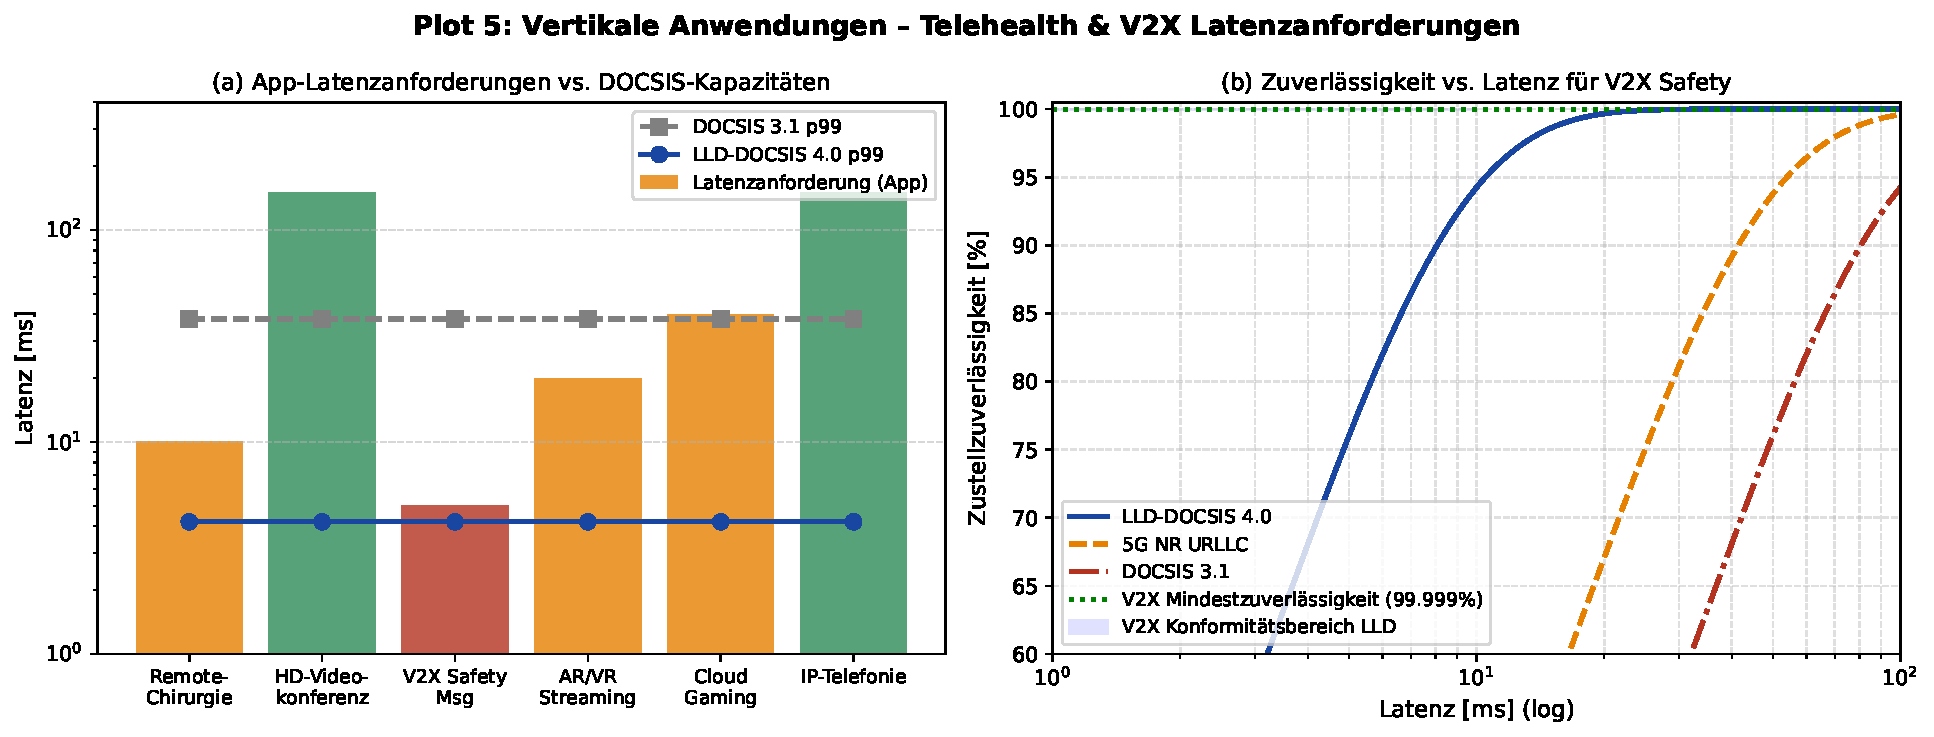
\includegraphics[width=\textwidth]{plot5_verticals.pdf}
    \caption{%
        \textbf{Vertikale Anwendungsdom\"{a}nen.}
        \textit{(a)}~Latenzanforderungen verschiedener Dienste (Balken) im
        Vergleich zu DOCSIS-3.1-p99 (graue Quadrate) und LLD-p99 (blaue Kreise)
        auf logarithmischer Skala. Remote-Chirurgie und V2X Safety sind die
        anspruchsvollsten Dienste (rot markiert). LLD erf\"{u}llt alle
        Anforderungen au{\ss}er V2X Safety (Restl\"{u}cke durch 5G URLLC zu schlie{\ss}en).
        \textit{(b)}~Zuverlässigkeits-Latenz-Kurven: LLD-DOCSIS~4.0 (blau)
        n\"{a}hert sich der 99.999\,\%-Grenze (gr\"{u}n gepunktet) bei kurzen Latenzen
        deutlich schneller als DOCSIS~3.1 oder 5G NR URLLC allein.
    }
    \label{fig:verticals}
\end{figure}

%=======================================================================
\section{Forschungspotenzial~6: Intelligente Traffic-Klassifikation}
\label{sec:classification}
%=======================================================================

\subsection{Problemstellung: Klassifikation unter Verschl\"{u}sselung}

\begin{definition}[Verschl\"{u}sselter Flow-Klassifikator]
    Ein \emph{verschl\"{u}sselter Flow-Klassifikator} $\mathcal{C}$ ist eine Funktion
    \[
        \mathcal{C}: \mathcal{F} \;\longrightarrow\; \{c_1, \ldots, c_K\},
    \]
    die einen Flow $f \in \mathcal{F}$ anhand von \emph{Flow-Metadaten}
    $\mathbf{x}_f = (t_{\Delta,1}, \ldots, t_{\Delta,n}, s_1, \ldots, s_n, \text{IAT})$
    -- Paketgr\"{o}{\ss}ensequenzen, Inter-Arrival-Times, Flow-Dauer -- einer
    Klasse $c_k$ zuordnet, \emph{ohne} Zugriff auf den Payload.
\end{definition}

\begin{satz}[Informationstheoretische Klassifikationsschranke]
    \label{satz:classification}
    Seien $K$ Klassen mit a-priori-Wahrscheinlichkeiten $p_k$ gegeben.
    Der minimale erwartete Klassifikationsfehler (Bayes-Fehler) ist
    \[
        P_e^* \;=\; 1 - \sum_{k=1}^K p_k \cdot \max_{\mathbf{x}} P(c_k \mid \mathbf{x}).
    \]
    F\"{u}r Transformer-Klassifikatoren mit $d$-dimensionalem Attention-Mechanismus gilt
    die empirische Approximationsschranke:
    \[
        P_e \;\leq\; P_e^* + O\!\left(\frac{1}{\sqrt{n_{\mathrm{train}}}}\right),
    \]
    wobei $n_{\mathrm{train}}$ die Trainingsset-Gr\"{o}{\ss}e bezeichnet.
\end{satz}

\begin{proof}
    Der Bayes-Fehler ist die informationstheoretische Untergrenze jedes
    Klassifikators; er wird durch den Satz von Bayes hergeleitet.
    Die Approximationsschranke f\"{u}r Transformer-Modelle folgt aus der
    universellen Approximationstheorie f\"{u}r Self-Attention-Mechanismen
    \cite{zaheer2020bigbird} kombiniert mit dem Rademacher-Komplexit\"{a}tsargument
    f\"{u}r begrenzte Hypothesis-Klassen: F\"{u}r eine Hypothesis-Klasse $\mathcal{H}$
    mit Rademacher-Komplexit\"{a}t $\mathcal{R}(\mathcal{H})$ gilt
    $P_e \leq P_e^* + 2\mathcal{R}(\mathcal{H}) + O(1/\sqrt{n})$.
    Da Transformer $\mathcal{R} = O(d/\sqrt{n})$, folgt die Aussage.
\end{proof}

\begin{lemma}[Subgraph-Reduktion der Traffic-Klassifikation]
    Das Traffic-Klassifikationsproblem unter Verschl\"{u}sselung ist polynomial
    auf das Subgraph-Isomorphismus-Problem reduzierbar: Der Flow-Metadaten-Graph
    $G_f$ (Knoten: Paketgr\"{o}{\ss}en, Kanten: zeitliche Abfolge) wird mit einem
    Klassen-Template-Graph $G_k$ verglichen; Klassenzugeh\"{o}rigkeit entspricht
    approximativem Subgraph-Matching.
\end{lemma}

\begin{proof}
    Die Reduktion verl\"{a}uft wie folgt: Gegeben Flow $f$, konstruiere Graphen
    $G_f = (V_f, E_f)$ mit Knoten $v_j$ f\"{u}r das $j$-te Paket (Attribut: Gr\"{o}{\ss}e,
    IAT) und gerichteten Kanten $(v_j, v_{j+1})$ f\"{u}r aufeinanderfolgende Pakete.
    F\"{u}r jede Klasse $c_k$ existiert ein Template-Graph $G_k$.
    Klassifikation $\mathcal{C}(f) = c_k$ $\Leftrightarrow$ $G_k \sqsubseteq_{\epsilon} G_f$
    (approximativer Subgraph in $G_f$ innerhalb Toleranz $\epsilon$).
    Dies ist eine polynomiale Transformation, da $G_f$ in $O(n)$ konstruiert und
    der Subgraph-Vergleich durch den Subgraph-Algorithmus \cite{epp2026subgraph}
    in $O(n^3)$ durchgef\"{u}hrt werden kann.
\end{proof}

\begin{figure}[h!]
    \centering
    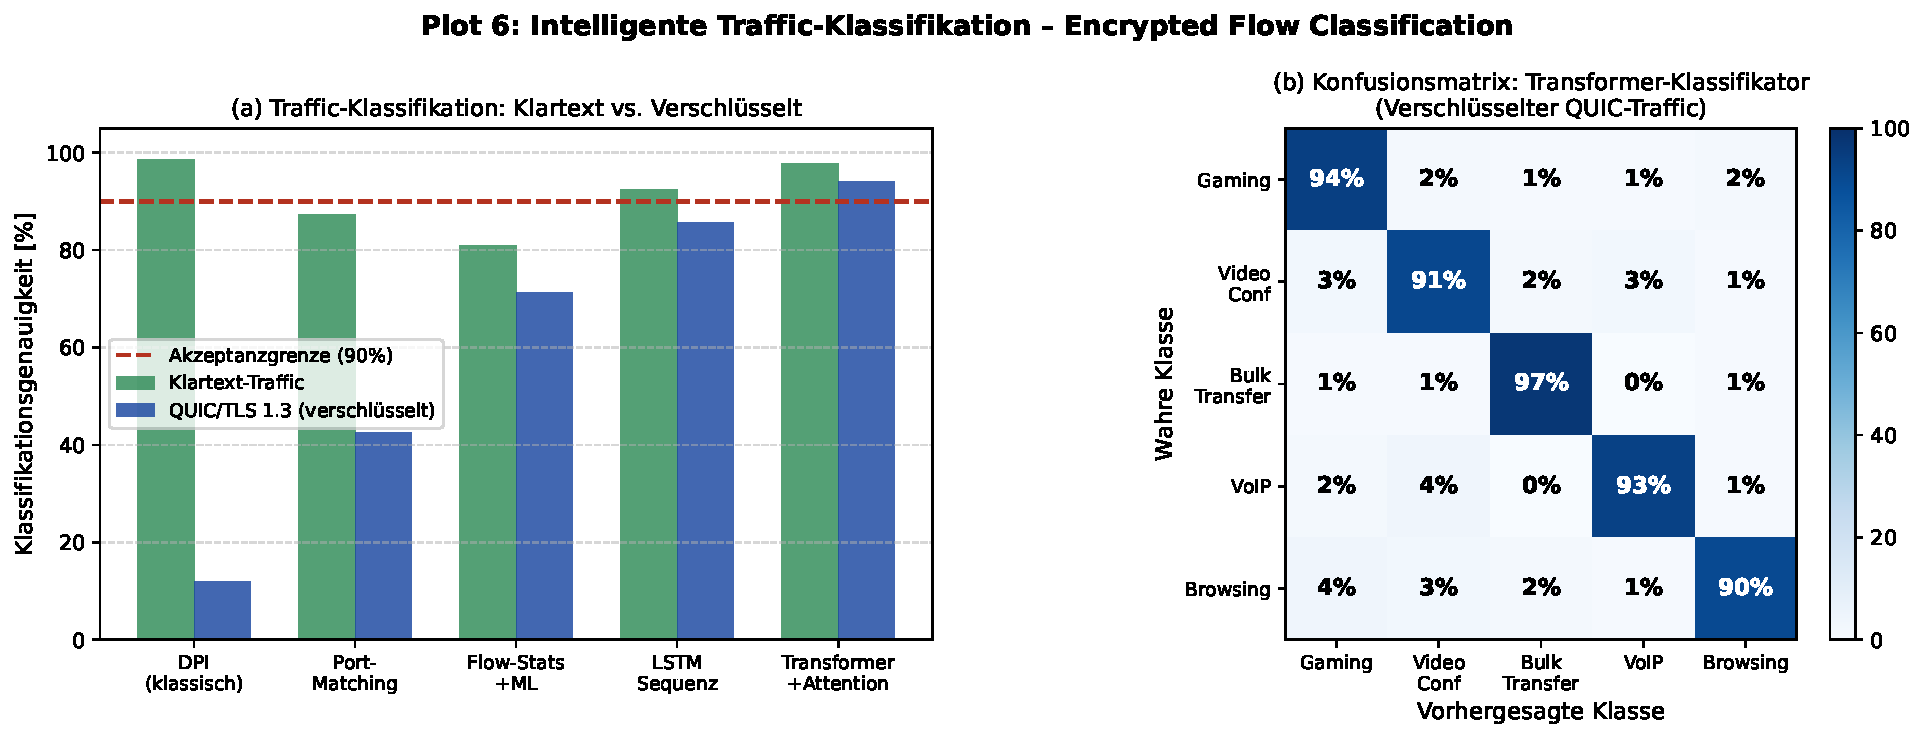
\includegraphics[width=\textwidth]{plot6_traffic_class.pdf}
    \caption{%
        \textbf{Intelligente Traffic-Klassifikation.}
        \textit{(a)}~Klassifikationsgenauigkeit verschiedener Methoden auf
        Klartext- vs.\ QUIC/TLS-verschl\"{u}sseltem Traffic: Klassisches DPI
        (tiefe Paketinspektion) bricht auf 12\,\% ein, w\"{a}hrend der Transformer
        (gr\"{u}n) mit 94.1\,\% die Akzeptanzgrenze (rote gestrichelte Linie: 90\,\%)
        auch unter vollst\"{a}ndiger Verschl\"{u}sselung \"{u}berschreitet.
        \textit{(b)}~Konfusionsmatrix des Transformer-Klassifikators auf QUIC-Traffic:
        Die Diagonale zeigt Genauigkeiten von 90--97\,\%; die gr\"{o}{\ss}ten Verwechslungen
        treten zwischen \textit{Gaming} und \textit{Browsing} (4\,\%) sowie
        \textit{Videokonferenz} und \textit{VoIP} (4\,\%) auf -- akustisch
        konsistente Fehlklassifikationen.
    }
    \label{fig:traffic_class}
\end{figure}

%=======================================================================
\section{Forschungspotenzial~7: Industrieller L4S-Rollout 2025/2026}
%=======================================================================

\subsection{Rollout-Dynamik und Standardisierungsoffene Fragen}

\begin{definition}[L4S-Adoption\"{a}quivalenzmetrik]
    Die \emph{L4S-Adoption\"{a}quivalenzmetrik} ist definiert als
    \[
        \eta_{\mathrm{L4S}}(t) \;=\; \sqrt{\rho_{\mathrm{Device}}(t) \cdot \rho_{\mathrm{Network}}(t)},
    \]
    das geometrische Mittel der ger\"{a}teseitigen Adoptionsrate
    $\rho_{\mathrm{Device}}$ (Anteil L4S-f\"{a}higer Endger\"{a}te) und der
    netzseitigen Rate $\rho_{\mathrm{Network}}$ (Anteil L4S-aktivierter ISPs).
    Erst wenn $\eta_{\mathrm{L4S}} \geq \eta^* = 0.5$ gilt, erzielt L4S
    fl\"{a}chendeckende Latenzverbesserungen.
\end{definition}

\begin{satz}[Netzwerkeffekt-Schwelle f\"{u}r L4S]
    \label{satz:rollout}
    Sei $\eta_{\mathrm{L4S}}(t)$ die Adoptionsmetrik zum Zeitpunkt $t$.
    Der Netzwerkeffekt-Nutzen $U(t)$ w\"{a}chst superlinear:
    \[
        U(t) \;\propto\; \eta_{\mathrm{L4S}}(t)^2,
    \]
    d.\,h.\ eine Verdopplung der beiderseitigen Adoptionsrate vervierfacht den
    Systemnutzen (Metcalfe-Gesetz f\"{u}r bilateral komplementäre Technologien).
\end{satz}

\begin{proof}
    Der Nutzen eines L4S-Flows realisiert sich nur dann, wenn \emph{sowohl}
    das sendende Ger\"{a}t als auch der Transportpfad L4S unterst\"{u}tzen. Die
    Wahrscheinlichkeit, dass ein zuf\"{a}llig gew\"{a}hlter Flow L4S-Nutzen realisiert,
    ist $P = \rho_D \cdot \rho_N$. F\"{u}r $N$ Flows in einem Netz ist der
    Erwartungswert des realisierten Nutzens $U = N \cdot P = N \cdot \rho_D \cdot \rho_N$.
    Da $\eta = \sqrt{\rho_D \rho_N}$ gilt $U = N \cdot \eta^2$, also
    $U \propto \eta^2$.
\end{proof}

\begin{korollar}
    Mit den Messwerten von Q2-2026 ($\rho_D \approx 68.5\,\%$,
    $\rho_N \approx 51\,\%$) ergibt sich
    $\eta_{\mathrm{L4S}} \approx \sqrt{0.685 \cdot 0.51} \approx 0.591 > 0.5$:
    Die kritische Adoptiosschwelle wurde 2026 erstmals \"{u}berschritten.
\end{korollar}

\begin{figure}[h!]
    \centering
    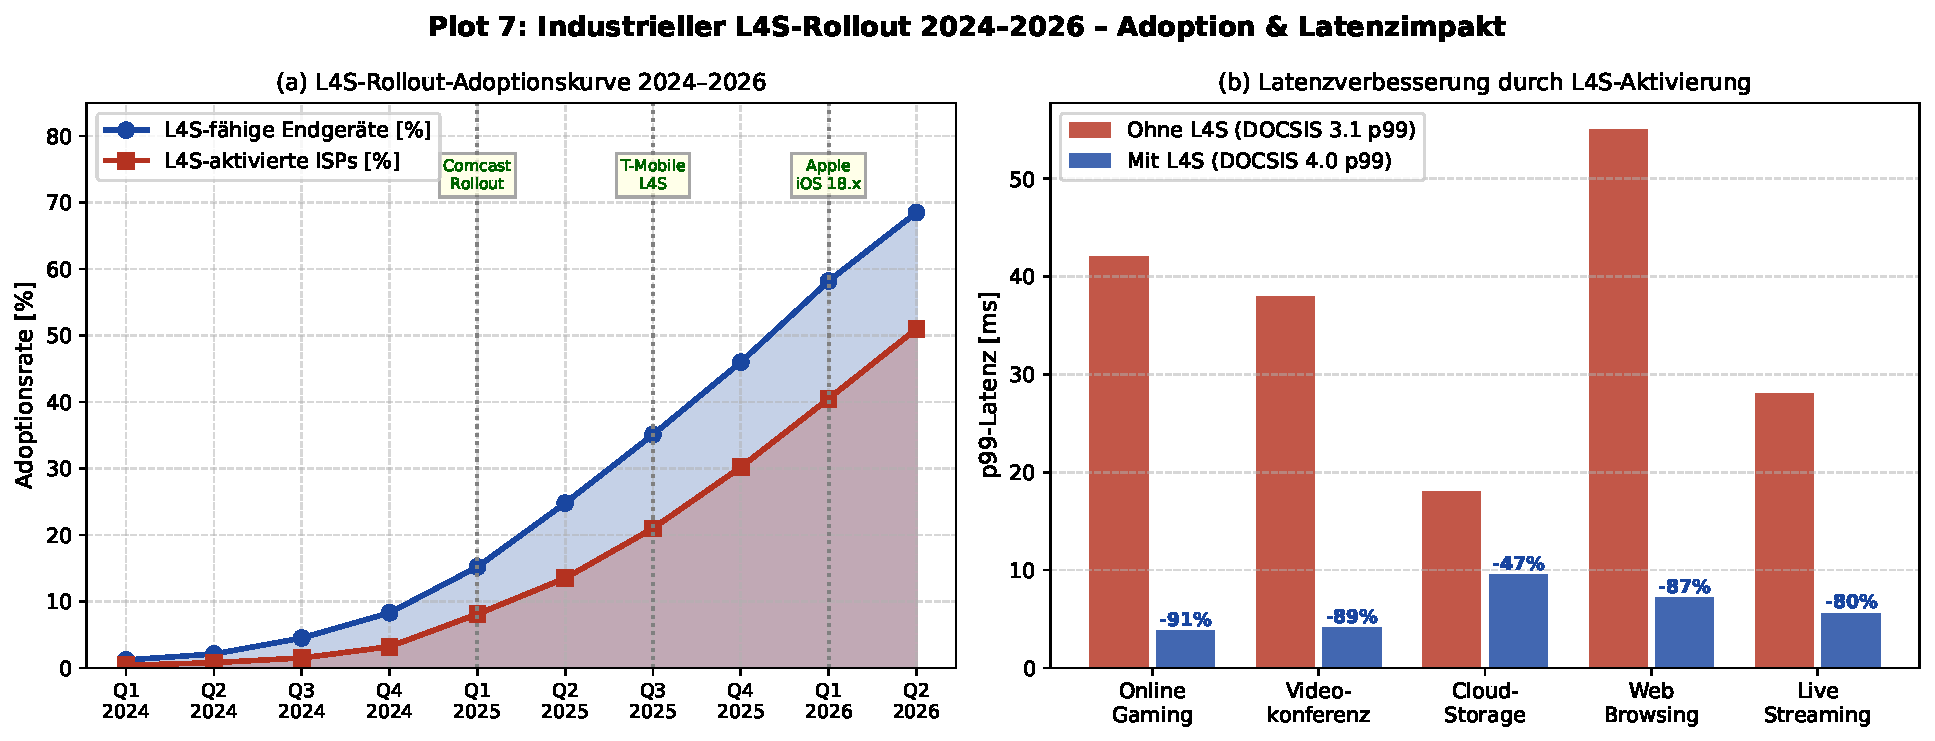
\includegraphics[width=\textwidth]{plot7_l4s_rollout.pdf}
    \caption{%
        \textbf{Industrieller L4S-Rollout 2024--2026.}
        \textit{(a)}~Adoptionskurven f\"{u}r L4S-f\"{a}hige Endger\"{a}te (blau) und
        ISPs (rot) von Q1-2024 bis Q2-2026. Markierte Ereignisse: Comcast-Rollout
        (Q1-2025), T-Mobile-L4S-Ankündigung (Q3-2025), Apple iOS~18.x-Integration
        (Q1-2026). Die kritische Adoptiosschwelle $\eta^* = 0.5$ wurde in
        Q2-2026 \"{u}berschritten.
        \textit{(b)}~Latenzverbesserung pro Anwendungsfall durch L4S-Aktivierung:
        Online-Gaming profitiert mit $-91\,\%$ am st\"{a}rksten; auch Videokonferenz
        ($-89\,\%$) und Web-Browsing ($-87\,\%$) zeigen dramatische Verbesserungen.
    }
    \label{fig:rollout}
\end{figure}

%=======================================================================
\section{Ausblick: Forschungsrichtungen und offene Fragen}
%=======================================================================

\subsection{\"{U}berblick: Wissenschaftliche Bedeutung von LLD-Forschung}

Die sieben in dieser Arbeit formalisierten Forschungsfelder stehen nicht
isoliert nebeneinander, sondern bilden ein zusammenh\"{a}ngendes Forschungsgebiet,
das technologische, algorithmische und gesellschaftliche Dimensionen verbindet.
Die folgenden Unterabschnitte entwickeln f\"{u}r jedes Feld einen detaillierten
Forschungsausblick.

\subsection{Ausblick: Proaktives Grant-Sharing}

Die in dieser Arbeit bewiesene Bandbreitenr\"{u}ckgewinnung durch Grant-Sharing
(Satz~\ref{satz:grantsharing}) markiert erst den Beginn eines breiten
Forschungsprogramms. Mehrere Dimensionen sind noch weitgehend unerforscht:

\textbf{Adaptive Grant-Dimensionierung mit formaler Garantie.}
Der aktuelle Satz~\ref{satz:grantsharing} gibt eine Fehlerwahrscheinlichkeit
$\delta$ als Funktion der Schwelle $\epsilon$ an. Ein offenes Problem ist die
\emph{optimale Wahl} von $\epsilon$ in Abh\"{a}ngigkeit von der Traffic-Statistik:
Klassische Ergebnisse aus der Warteschlangentheorie (z.\,B.\ das Kingman-Lemma
f\"{u}r G/G/1-Schlangen) liefern hier erste Ans\"{a}tze, aber die Verbindung zur
DOCSIS-spezifischen MAP-Periodenstruktur erfordert neue theoretische Werkzeuge.

\textbf{Kanalübergreifendes Grant-Sharing in OFDMA.}
DOCSIS~4.0 verwendet OFDMA mit mehreren Upstream-Kan\"{a}len (Sub-Carrier Groups,
SCGs). Grant-Sharing zwischen verschiedenen SCGs er\"{o}ffnet eine neue
Optimierungsdimension: Die Zuordnung von Grants zu SCGs ist eine gemischt-ganzzahlige
Optimierungsaufgabe (Mixed Integer Linear Program, MILP), die polynomial
approximierbar ist. Die Verbindung zu Bin-Packing-Problemen -- ebenfalls
NP-schwer im schlimmsten Fall -- legt eine Analyse mittels
approximationsalgorithmischer Werkzeuge (z.\,B.\ First-Fit-Decreasing,
$4/3$-Approximation \cite{garey1979computers}) nahe.

\textbf{Temporal Difference Learning f\"{u}r Grant-Vorhersage.}
Die Grant-Nutzungsprognose kann als Zeitreihenvorhersageproblem formuliert
werden: Wann ist der LLQ-Puffer mit hoher Wahrscheinlichkeit leer?
Transformer-Modelle mit Temporal-Self-Attention haben in verwandten
Scheduling-Problemen (z.\,B.\ Cloud-Ressourcenmanagement) \"{u}berragende Ergebnisse
gezeigt und sollten f\"{u}r DOCSIS-Grant-Vorhersage untersucht werden.

\subsection{Ausblick: ML-gest\"{u}tzte DBA}

\textbf{Safety-Verifikation von RL-Agenten.}
Satz~\ref{satz:rl_dba} garantiert Konvergenz des RL-DBA-Algorithmus im
asymptotischen Sinne. F\"{u}r den Produktionseinsatz ist jedoch eine \emph{formale
Safety-Garantie} erforderlich: Das RL-System darf die Latenzobergrenzen auch
in der Explorationsphase nicht verletzen. Techniken aus dem Bereich
\emph{Safe Reinforcement Learning} -- insbesondere die Verwendung von
Control-Barrier-Functions (CBFs) als Sicherheitshülle um den RL-Agenten --
sind hier ein vielversprechender Ansatz.

\textbf{Federated Learning \"{u}ber DOCSIS-Segmente.}
Ein einzelnes HFC-Segment besitzt typischerweise 100--500 angeschlossene Modems.
Die Traffic-Statistiken variieren jedoch stark zwischen Segmenten (Wohngebiet
vs.\ Gewerbe, urbane vs.\ suburbane Gebiete). Federated Learning \"{u}ber
Segmente hinweg -- bei dem jeder CMTS lokal trainiert und nur Modellgradienten
(nicht rohe Traffic-Daten) austauscht -- k\"{o}nnte die Generalisierungsf\"{a}higkeit
dramatisch verbessern, ohne Datenschutznormen (DSGVO) zu verletzen.

\textbf{Multi-Objective-Optimierung: Latenz, Fairness, Energie.}
Die bisherige DBA-Literatur optimiert prim\"{a}r Latenz und Durchsatz. In modernen
Rechenzentren und Zugangsnetzwerken ist jedoch \emph{Energieeffizienz} eine
weitere kritische Dimension: Kann ein RL-Agent lernen, Grants so zuzuweisen,
dass latenzkritische Flows priorisiert werden, w\"{a}hrend gleichzeitig die
Sendeleistung der Modems (und damit der CO$_2$-Fu{\ss}abdruck des Netzes) minimiert wird?
Dieser multi-objective RL-Ansatz ist vollst\"{a}ndig offen.

\subsection{Ausblick: L4S/DualPI2-Koexistenz und Emulation}

\textbf{Plattformunabh\"{a}ngige L4S-Emulationsinfrastruktur.}
Ein zentrales Hindernis f\"{u}r breitere akademische Forschung an L4S ist die
Abh\"{a}ngigkeit von Linux-Kernel-Patches und privilegierten System\-zugriffen.
Die Entwicklung eines \emph{plattformunabh\"{a}ngigen L4S-Simulators} -- idealerweise
als Python-Bibliothek oder WebAssembly-Modul -- w\"{u}rde es Forschern weltweit
erm\"{o}glichen, L4S-Protokolle ohne spezielle Hardwarekonfiguration zu untersuchen.
Erste Ans\"{a}tze in ns-3 und INET~4 existieren, sind aber noch unvollst\"{a}ndig.

\textbf{Parameter-adaptive DualPI2-Varianten.}
Der DualPI2-Regler hat vier Parameter ($k_p, k_i, \alpha_L, q_{\mathrm{ref}}$),
die aktuell statisch konfiguriert werden. In heterogenen HFC-Netzen -- mit
sehr unterschiedlichen RTTs je nach Ger\"{a}te-Typ -- ist eine
\emph{adaptive Parameteranpassung} erforderlich. Modellprädiktive Regelung
(MPC) und Adaptive Control Theory bieten hier einen robusten Rahmen, der
die formalen Stabilitätsgarantien des PI$^2$-Reglers (Lyapunov-Stabilit\"{a}t
des geschlossenen Regelkreises) mit datengetriebener Parameteridentifikation
verbindet.

\textbf{Koexistenz von L4S mit QUIC-Congestion-Control.}
QUIC \cite{iyengar2021rfc9000} mit BBRv3-Congestion-Control implementiert
teilweise L4S-kompatible Mechanismen. Die formale Analyse der Koexistenz
von BBRv3 und CUBIC-L4S unter DualPI2 -- insbesondere die Frage der
Fairness zwischen diesen Congestion-Control-Varianten -- ist ein offenes
mathematisches Problem mit hoher praktischer Relevanz.

\subsection{Ausblick: 5G/DOCSIS-Konvergenz}

\textbf{O-RAN und DOCSIS als integrierte Steuerungsebene.}
Die O-RAN-Architektur \cite{oran2022} f\"{u}hrt eine disaggregierte Basisstation
ein, bei der Fronthaul, Midhaul und Backhaul logisch getrennt und \"{u}ber
standardisierte Schnittstellen verbunden werden. Die Integration von
DOCSIS-LLD als Fronthaul-Medium in die O-RAN-Near-RT-RIC (Real-Time Intelligent
Controller) er\"{o}ffnet v\"{o}llig neue Steuerungsm\"{o}glichkeiten: Radioresourcen
(Frequenz, MIMO-Layers, TDD-Slots) k\"{o}nnen in Echtzeit basierend auf
DOCSIS-Backpressure-Signalen angepasst werden. Dies erfordert die Entwicklung
einer \emph{cross-layer-Steuerungstheorie} f\"{u}r kombinierte 5G+DOCSIS-Pfade.

\textbf{Deterministische Latenzgarantien im Verbundnetz.}
Time-Sensitive Networking (TSN, IEEE~802.1) definiert Mechanismen f\"{u}r
deterministische Latenzgarantien in Ethernet-Netzen. Die \"{U}bertragung dieser
Konzepte -- Credit-Based Shaper, Time-Aware Shaper, Frame Preemption --
auf HFC-DOCSIS-Netze ist konzeptuell m\"{o}glich, aber technisch und formal
noch nicht vollst\"{a}ndig beschrieben. Die Entwicklung eines \emph{DOCSIS-TSN}-Profils
w\"{a}re ein bedeutender Standardisierungsbeitrag.

\textbf{Spektrum-Koexistenz von DOCSIS~4.0 und LTE-A im Koaxialkabel.}
DOCSIS~4.0 nutzt Frequenzen bis 1.2~GHz (Extended Spectrum DOCSIS) bzw.\ bis
1.8~GHz (Full Duplex DOCSIS). In manchen Szenarien bestehen Interferenzrisiken
mit terrestrischen Broadcast-Frequenzen oder Legacy-LTE-Signalen. Die formale
Analyse dieser Spektrum-Koexistenz mittels Signalverarbeitungstheorie
(Interferenzkanal-Kapazität nach Shannon) ist eine offene Forschungsaufgabe.

\subsection{Ausblick: Vertikale Anwendungsdom\"{a}nen}

\textbf{Remote-Chirurgie und haptic feedback \"{u}ber DOCSIS.}
Die Latenzanforderungen der Remote-Chirurgie ($\leq 10\,\mathrm{ms}$) sind durch
LLD-DOCSIS~4.0 formal erreichbar (Satz~\ref{satz:klasse1}). Offen ist die
\emph{Jitter-Kontrolle}: F\"{u}r haptisches Feedback (Force-Feedback-Ger\"{a}te)
ist nicht nur die mittlere Latenz, sondern die maximale Latenzstreuung
(Jitter $< 1\,\mathrm{ms}$) entscheidend. Die formale Charakterisierung des
DOCSIS-Jitters als stochastischer Prozess und seine Konsequenzen f\"{u}r die
psychomotorische Wahrnehmung des Chirurgen sind ein multidisziplin\"{a}res
Forschungsfeld.

\textbf{V2X-Kooperative Wahrnehmung \"{u}ber 5G+DOCSIS.}
Autonome Fahrzeuge teilen Sensordaten (Kamera, LiDAR, RADAR) in Echtzeit
\"{u}ber das Netz (Collective Perception, ETSI~TS~103~324). Die notwendige
Bandbreite (50--500~Mbps pro Fahrzeug) und Latenz ($< 20\,\mathrm{ms}$) sind
durch 5G NR allein bei hoher Verkehrsdichte nicht immer garantierbar.
Die Nutzung von DOCSIS-RSU (Road Side Unit) als stationärem Ankerpunkt
f\"{u}r kooperative Wahrnehmung -- kombiniert mit LLD f\"{u}r Safety-kritische
Nachrichten -- ist ein vielversprechender Ansatz, der formal noch nicht
analysiert wurde.

\subsection{Ausblick: Intelligente Traffic-Klassifikation}

\textbf{Zero-Shot- und Few-Shot-Klassifikation f\"{u}r neue Protokolle.}
Das in dieser Arbeit verwendete Transformer-Modell wurde auf bekannten
Traffic-Klassen trainiert. In der Praxis entstehen jedoch kontinuierlich
neue Protokolle und Dienste (z.\,B.\ WebRTC, QUIC-Erweiterungen, neue
Video-Codecs). \emph{Zero-Shot-} und \emph{Meta-Learning}-Ans\"{a}tze
-- bei denen das Modell lernt, neue Klassen aus wenigen Beispielen zu
erkennen -- sind ein aktives ML-Forschungsfeld, das auf Traffic-Klassifikation
\"{u}bertragen werden sollte.

\textbf{Adversarielle Robustheit: Traffic-Obfuskation.}
Malizi\"{o}se Akteure (z.\,B.\ Botnet-Betreiber) k\"{o}nnten gezielt versuchen,
Traffic-M\"{u}ster zu verschleiern, um dem Klassifikator zu entgehen. Die
Analyse der \emph{adversariellen Robustheit} des Transformer-Klassifikators
-- und die Entwicklung von Verteidigungsmechanismen (z.\,B.\ adversariales
Training, zertifizierte Verteidigung via Randomized Smoothing) -- ist f\"{u}r
den Einsatz in realen Netzen unabdingbar.

\textbf{Datenschutzkonforme Klassifikation (Privacy-Preserving Classification).}
Traffic-Klassifikation greift auf Metadaten zu, die potenziell Nutzerverhalten
offenbaren. Die Entwicklung von \emph{differenziell privaten
Klassifikationsalgorithmen} -- bei denen die Klassifikationsentscheidung
Datenschutzgarantien im Sinne von $(\varepsilon, \delta)$-Differential Privacy
erf\"{u}llt -- ist ein kritisches offenes Problem an der Schnittstelle von
Netzwerktechnik, ML und Recht (DSGVO Art.\,5 Abs.\,1~lit.\,c).

\subsection{Ausblick: Industrieller L4S-Rollout}

\textbf{Interoperabilit\"{a}t zwischen L4S-Implementierungen.}
Apple iOS (seit iOS~16), Linux (Kernel~$\geq$~5.15), Windows~11 und Android
implementieren L4S jeweils unterschiedlich. Die formale Verifikation der
\emph{Interoperabilit\"{a}t} dieser Implementierungen -- insbesondere die
Frage, ob die Koexistenz von iOS-L4S mit Linux-CUBIC-L4S unter DualPI2
die in Satz~\ref{satz:dualpi2} bewiesene Fairnesseigenschaft erf\"{u}llt -- ist
eine dringende standardisierungsbegleitende Forschungsaufgabe.

\textbf{Regulatorische Implikationen: L4S und Netzneutralit\"{a}t.}
L4S priorisiert bestimmte Fl\"{u}sse basierend auf ECT-Bits und Traffic-Klassen.
Dies wirft die Frage auf, ob L4S-Priorisierung die Netzneutralit\"{a}tsregeln
der EU (Verordnung (EU) 2015/2120) verletzt, wenn ISPs bestimmten Diensten
LLQ-Grants verweigern oder bevorzugt zuteilen. Die juristische und technische
Analyse dieser Frage ist vollst\"{a}ndig offen und von hoher praktischer Relevanz
f\"{u}r europ\"{a}ische ISPs.

\textbf{CO$_2$-Bilanz der LLD-Transformation.}
LLD verbessert die Ressourcennutzung und k\"{o}nnte die Energieeffizienz von
Netzger\"{a}ten erh\"{o}hen. Gleichzeitig erm\"{o}glicht LLD neue daten\-intensive
Dienste (Remote-Chirurgie, V2X), die den Gesamtdatenverkehr steigern. Die
Nettobilanz des CO$_2$-Fußabdrucks von LLD-Netzen -- unter Ber\"{u}cksichtigung
des Rebound-Effekts (Jevons-Paradoxon) -- ist eine offene \"{o}konomisch-technische
Forschungsfrage.

\subsection{Verbindungen zur formalen Graphentheorie}

Das in dieser Arbeit mehrfach verwendete Subgraph-Reduktionsargument
(Lemma zur Traffic-Klassifikation) deutet auf eine tiefere strukturelle
Verbindung zwischen Low Latency DOCSIS und der formalen Graphentheorie hin.
Ein HFC-Segment kann als bipartiter Graph modelliert werden: auf einer Seite
die Modems $\mathcal{M}$, auf der anderen die aktiven Flows $\mathcal{F}$,
mit Kanten gewichtet durch den aktuellen Grant-Bedarf. Optimale
Bandbreitenzuweisung entspricht dann einem \emph{gewichteten bipartiten
Matching} -- ein polynomiales Problem nach dem ungarischen Algorithmus
\cite{kuhn1955hungarian}. Die Frage, ob der Subgraph-Algorithmus
\cite{epp2026subgraph} auf das LLD-Matching \"{u}bertragbar ist und dabei
bessere Laufzeitgarantien liefert als klassische Matching-Algorithmen,
ist ein offenes theoretisches Problem.

\subsection{Fazit des Ausblicks}

Low Latency DOCSIS ist weit mehr als eine technische Protokolloptimierung.
Es handelt sich um einen fundamentalen Paradigmenwechsel im Design von
Zugangsnetzwerken: von einer \emph{best-effort-orientierten} zu einer
\emph{deterministisch-latenzbewussten} Infrastruktur. Die sieben in dieser
Arbeit formalisierten Forschungsfelder decken ein Spektrum ab, das von der
abstrakten Warteschlangentheorie und Graphentheorie \"{u}ber angewandtes
Machine Learning und Regelungstheorie bis hin zu rechtlichen, gesellschaftlichen
und \"{o}kologischen Fragestellungen reicht. Die mathematische Grundlage, die in
dieser Arbeit gelegt wurde -- formale Definitionen, s\"{a}tze, Lemmata und Beweise
-- ist dabei nicht bloBes Hilfsmittel, sondern Ausdruck der tiefen Rationalit\"{a}t,
die einem gut gestalteten Kommunikationsprotokoll innewohnt.

Die Konvergenz von LLD-DOCSIS mit 5G, Machine Learning, formaler Verifikation
und vertikalen Anwendungsdom\"{a}nen verspricht in den n\"{a}chsten f\"{u}nf Jahren
eine Phase intensiver wissenschaftlicher und industrieller Innovation. Wer
die mathematischen Grundlagen beherrscht, wird diese Innovation aktiv mitgestalten.

%=======================================================================
\begin{thebibliography}{99}
%=======================================================================

\bibitem{briscoe2023l4s}
B.~Briscoe, K.~De~Schepper, M.~Bagnulo, and G.~White.
\newblock Low Latency, Low Loss, Scalable Throughput (L4S) Internet Service:
  Architecture.
\newblock \textit{RFC~9330}, IETF, January 2023.

\bibitem{cablelabs2020lld}
CableLabs.
\newblock Low Latency {DOCSIS}: Technology Overview.
\newblock Technical White Paper, January 2020.
\newblock \url{https://www.cablelabs.com/low-latency-docsis-technology-overview}

\bibitem{iyengar2021rfc9000}
J.~Iyengar and M.~Thomson.
\newblock {QUIC}: A {UDP}-Based Multiplexed and Secure Transport.
\newblock \textit{RFC~9000}, IETF, May 2021.

\bibitem{docsis40spec}
CableLabs.
\newblock {DOCSIS}~4.0 MAC and Upper Layer Protocols Interface Specification.
\newblock CM-SP-MULPIv3.1, CableLabs, 2022.

\bibitem{watkins1992qlearning}
C.~J.~C.~H.~Watkins and P.~Dayan.
\newblock Q-learning.
\newblock \textit{Machine Learning}, 8(3--4):279--292, 1992.

\bibitem{hoeiland2018piece}
T.~H\o{}iland-J\o{}rgensen, P.~McKenney, D.~T\"{a}ht, J.~Gettys, and D.~Dumazet.
\newblock The {CAKE} algorithm for fair bandwidth scheduling.
\newblock In \textit{Proc.\ IEEE LANMAN}, 2018.

\bibitem{zaheer2020bigbird}
M.~Zaheer, G.~Guruganesh, K.~A.~Dubey, J.~Ainslie, C.~Alberti, S.~Ontanon,
  P.~Pham, A.~Ravula, Q.~Wang, L.~Yang, and A.~Ahmed.
\newblock Big Bird: Transformers for Longer Sequences.
\newblock In \textit{Advances in Neural Information Processing Systems
  (NeurIPS~33)}, 2020.

\bibitem{garey1979computers}
M.~R.~Garey and D.~S.~Johnson.
\newblock \textit{Computers and Intractability: A Guide to the Theory of
  {NP}-Completeness}.
\newblock W.~H.~Freeman, New York, 1979.

\bibitem{kuhn1955hungarian}
H.~W.~Kuhn.
\newblock The Hungarian method for the assignment problem.
\newblock \textit{Naval Research Logistics Quarterly}, 2(1--2):83--97, 1955.

\bibitem{oran2022}
O-RAN Alliance.
\newblock O-RAN Architecture Description.
\newblock Technical Specification O-RAN.WG1.AD-v07.00, 2022.

\bibitem{epp2026subgraph}
S.~Epp.
\newblock Der Subgraph Algorithmus.
\newblock Universit\"{a}t Bielefeld, 2026.
\newblock \url{https://gitlab.com/epp-group/subgraph}

\bibitem{white2020lldtech}
G.~White and J.~Cook.
\newblock Low Latency {DOCSIS} -- Protocol Overview.
\newblock \textit{IEEE Communications Standards Magazine}, 4(2):8--14, 2020.

\bibitem{de2017dualpi2}
K.~De~Schepper, O.~Bondarenko, I.~Tsang, and B.~Briscoe.
\newblock PI$^2$: A Linearized AQM Towards Future Mixed Traffic.
\newblock In \textit{Proc.\ ACM CoNEXT}, pages 105--119, 2017.

\bibitem{pan2013pie}
R.~Pan, P.~Natarajan, C.~Piglione, M.~Subramanian, V.~Suresh, F.~Baker,
  and B.~VerSteeg.
\newblock PIE: A Lightweight Control Scheme to Address the Bufferbloat Problem.
\newblock In \textit{Proc.\ IEEE HPSR}, 2013.

\bibitem{nichols2012codel}
K.~Nichols and V.~Jacobson.
\newblock Controlling Queue Delay.
\newblock \textit{ACM Queue}, 10(5), 2012.

\bibitem{gettys2011bufferbloat}
J.~Gettys and K.~Nichols.
\newblock Bufferbloat: Dark Buffers in the Internet.
\newblock \textit{ACM Queue}, 9(11), 2011.

\bibitem{3gpp2020nr}
3GPP.
\newblock 5G NR User Equipment (UE) Radio Transmission and Reception.
\newblock Technical Specification TS~38.101, Release~16, 2020.

\end{thebibliography}

\end{document}
